%----------------------------------------------------------------------------
\chapter{\istio}
%----------------------------------------------------------------------------
A modern alkalmazásokat jellemzően mikroszolgáltatások elosztott gyűjteményeiként architektúrázzák, amelyek mindegyike valamilyen különálló üzleti funkciót lát el.
A szolgáltatásháló egy dedikált infrastrukturális réteg, amelyet hozzáadhat az alkalmazásaihoz.
Lehetővé teszi, hogy átlátható módon adjon hozzá olyan képességeket, mint a megfigyelhetőség, a forgalomirányítás és a biztonság, anélkül, hogy azokat a saját kódjához kellene hozzáadnia.
A ''szolgáltatásháló'' kifejezés leírja mind a minta megvalósításához használt szoftver típusát, mind pedig a szoftver használata során létrehozott biztonsági vagy hálózati tartományt.

Ahogy az elosztott szolgáltatások telepítése, például egy Kubernetes-alapú rendszerben, egyre nagyobb és összetettebb lesz, egyre nehezebbé válhat a megértése és kezelése. Követelményei közé tartozhat a felderítés, a terheléselosztás, a hibaelhárítás, a metrikák és a felügyelet.
A szolgáltatásháló gyakran olyan összetettebb üzemeltetési követelményekkel is foglalkozik, mint az A/B tesztelés, a kanáris telepítések, a forgalomkorlátozás, a hozzáférés-szabályozás, a titkosítás és a végponttól végpontig tartó hitelesítés.

Az elosztott alkalmazást a szolgáltatások közötti kommunikáció teszi lehetővé.
Ennek a kommunikációnak az útválasztása mind az alkalmazás cluster-én belül, mind pedig azok között egyre összetettebbé válik a szolgáltatások számának növekedésével.
Az Istio segít csökkenteni ezt a komplexitást, miközben megkönnyíti a fejlesztőcsapatok dolgát.

\section{Istio}
Az Istio a fejlesztők és az üzemeltetők előtt álló kihívásokat kezeli egy elosztott vagy mikroszolgáltatási architektúrával.
Akár a jelenlegi rendszerből építkezik, akár a nulláról vagy a meglévő alkalmazások felhőalapúvá történő migrálásáról, az Istio tud segíteni.

Az Istio egy nyílt forráskódú szolgáltatásháló, amely átláthatóan rétegződik a meglévő elosztott alkalmazásokra.
Az Istio fejlett funkciói egységes és hatékonyabb módot biztosítanak a szolgáltatások biztosítására, összekapcsolására és felügyeletére.
Az Istio az út a terheléselosztáshoz, a szolgáltatások közötti hitelesítéshez és a felügyelethez - kevés vagy semmilyen szolgáltatási kódváltoztatással.

\newpage

Kiforrott control plane-je létfontosságú funkciókat biztosít, többek között:

\begin{itemize}
    \item Biztonságos szolgáltatások közötti kommunikáció egy cluster-ben TLS-titkosítással, erős identitásalapú hitelesítést és engedélyezést.
    \item Automatikus terheléselosztást a HTTP, gRPC, WebSocket és TCP forgalomhoz.
    \item A forgalom viselkedésének finomra szabott vezérlését gazdag útválasztási szabályokkal, újbóli próbálkozásokkal, meghibásodásokkal és hibainjektálással.
    \item Beilleszthető házirend-réteget és konfigurációs API-t, amely támogatja a hozzáférés-szabályozást, a sebességkorlátozást és a kvótákat.
    \item Automatikus mérőszámokat, naplókat és nyomkövetést a cluster-en belüli összes forgalomra vonatkozóan, beleértve a cluster be- és kilépési pontjait is.
\end{itemize}

Az Istio-t bővíthetőségre tervezték, és a telepítési igények széles skáláját képes kezelni.
Az Istio control plane a Kubernetes-en fut, és az adott cluster-ben telepített alkalmazásokat hozzáadhatja a hálójához (későbbiekben mesh), a mesh-t kiterjesztheti más cluster-ekre, vagy akár virtuális gépeket és más a Kubernetes-en kívül futó végpontokat is csatlakoztathat.
A közreműködők, partnerek, integrációk és disztribútorok nagy ökoszisztémája az Istio-t a legkülönfélébb helyzetekre bővíti és hasznosítja.
Az Istio-t telepítheti saját maga, vagy számos gyártó rendelkezik olyan termékekkel, amelyek integrálják az Istio-t és kezelik azt a felhasználó számára.

Az Istio két komponensből áll: az adatsíkból (későbbiekben data plane) és a vezérlési síkból (későbbiekben control plane).
A data plane a szolgáltatások közötti kommunikációt jelenti.
Service Mesh nélkül a hálózat nem érti az átküldött forgalmat, és nem tud döntéseket hozni az alapján, hogy milyen típusú forgalomról van szó, vagy hogy kitől vagy kihez érkezik.
A Service Mesh egy proxy segítségével elfogja az összes hálózati forgalmat, és a felhasználó által beállított konfiguráció alapján lehetővé teszi az alkalmazásfüggő funkciók széles körét.
Az Envoy proxy minden olyan szolgáltatással együtt kerül telepítésre, amelyet a cluster-ben elindít, vagy a virtuális gépeken futó szolgáltatások mellett fut.
A control plane átveszi a kívánt konfigurációt és a szolgáltatásokról alkotott nézetét, és dinamikusan programozza a proxy-kiszolgálókat, frissítve azokat, amint a szabályok vagy a környezet változik \cite{istioSM}.

\begin{figure}[ht]
    \centering
         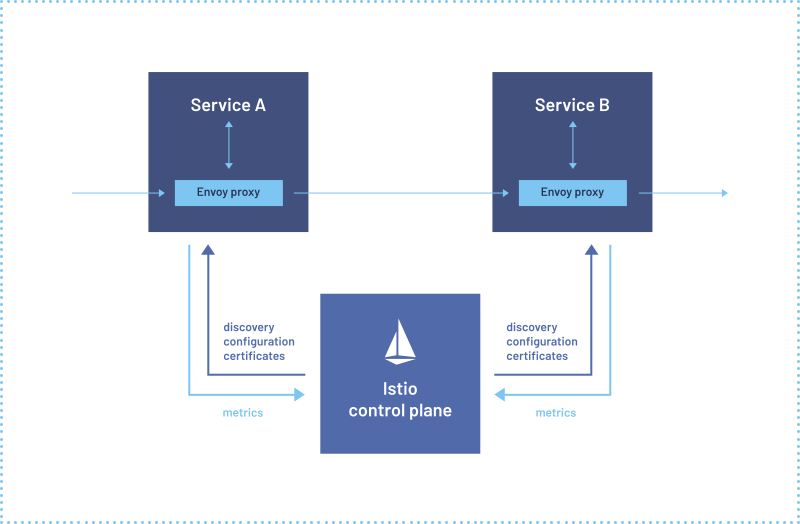
\includegraphics[width=1.0\textwidth]{figures/istio/service-mesh.png}
          \caption{Istio rendszer belső kommunikációjának ábrázolása \cite{istioSM}.}
           \label{service-mesh}
\end{figure}

\section{Istio operátor}
Az Istio-operator egy olyan egyéni erőforrást definiál, amely leírja az Istio telepítés kívánt állapotát.
Tartalmazza az összes szükséges konfigurációs értéket, és ha ezek közül egy vagy több megváltozik, az operátor automatikusan összehangolja a komponensek állapotát az új kívánt állapotnak megfelelően.

Az Istio-operátor lehetővé teszi a távoli konfigurációt futtató Kubernetes control plane-ek számára, hogy egyetlen Istio control plane-hez csatlakozzanak.
Az operátor kezeli az Istio komponensek távoli cluster-ekre történő telepítését, és olyan szinkronizációs mechanizmust ad, amely hozzáférést biztosít az Istio központi komponenseihez a távoli cluster-ekről.
Automatikusan nyomon követi azokat a névtereket, ahol az automatikus sidecar-injection engedélyezve van, így központilag kezelheti a funkciókat ahelyett, hogy egyesével kellene a névtereket felcímkézni \cite{banzaicloudOp}.

\begin{figure}[ht]
    \centering
         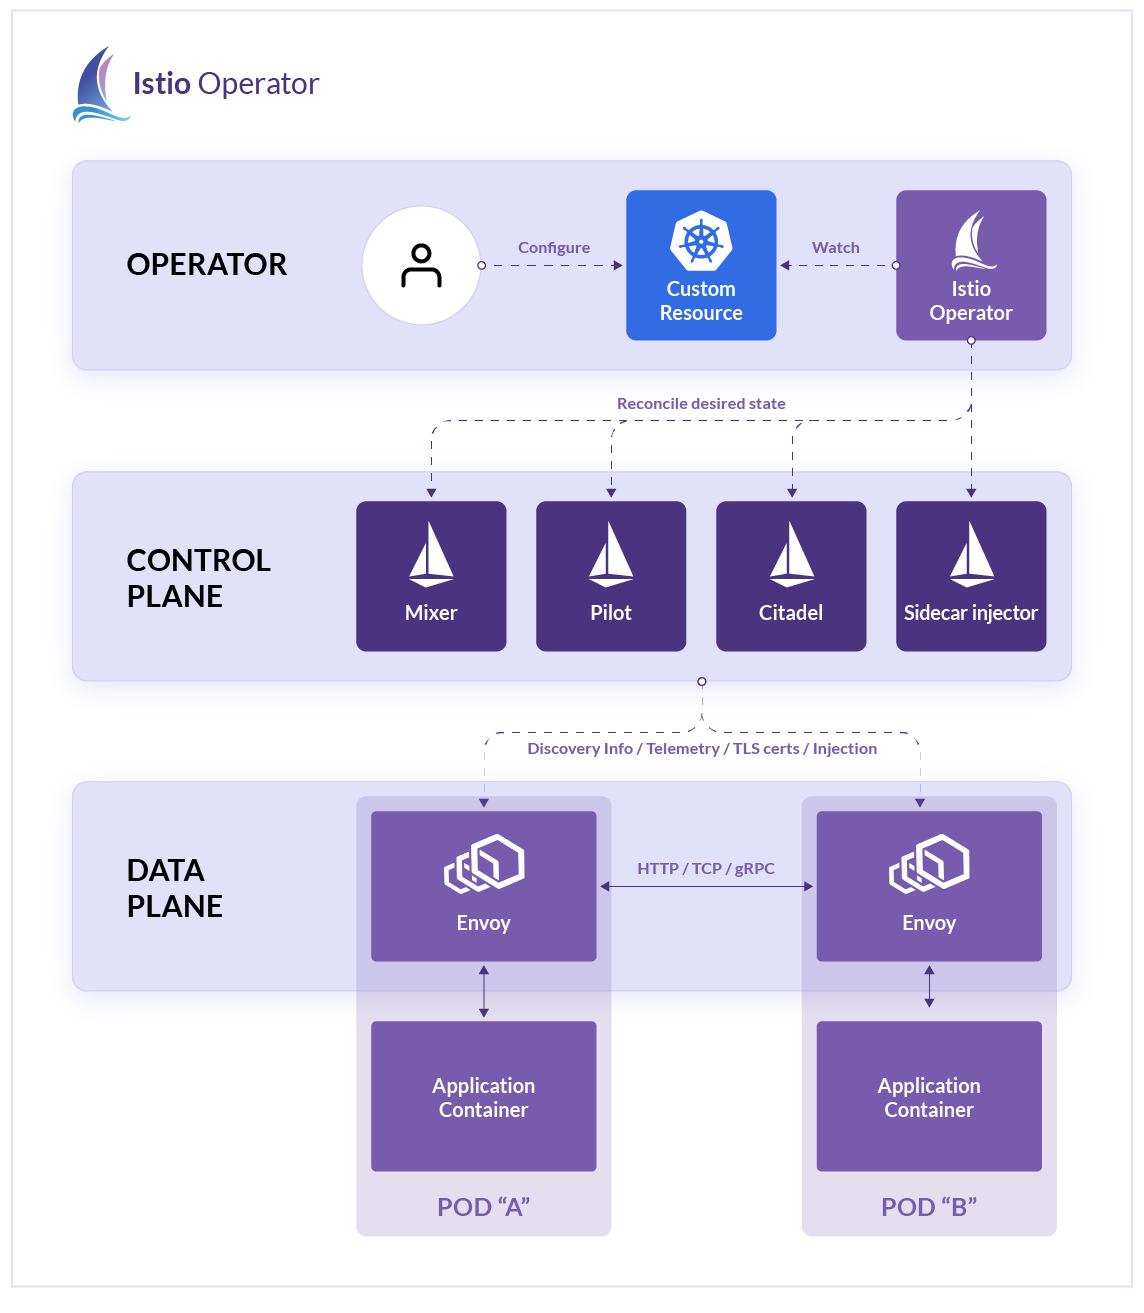
\includegraphics[width=0.9\textwidth]{figures/kubernetes/operator-overview.png}
          \caption{Istio operátor vizualizálása \cite{banzaicloudOp}.}
           \label{operator-overview}
\end{figure}

\section*{Cisco Istio operátor}
Az Istio csapat által fejlesztett Istio operátor nem bizonyult elegendőnek a Calisti Service Mesh Manager (SMM) termékének fejlsztése közben, így fork-olták és kibővítették azt.
Az SMM segít telepíteni, frissíteni, és menedzselni az Service Mesh-t és további egyéb eszközöket is nyújt:
\begin{itemize}
    \item Webes dashboard felület biztosítása.
    \item Automatikus multi cluster támogatás.
    \item Topológiai gráf megjelenítése.
    \item mTLS menedzsment.
    \item Virtuálisgép integrációja.
    \item stb...
\end{itemize}

\section{Multi cluster}
A több cluster-es (későbbiekben multi-cluster) Kubernetes egy olyan telepítési módszer, amely két vagy több cluster-ből áll.
Ez a telepítési módszer rendkívül rugalmas. Lehetnek cluster-ek ugyanazon a fizikai gépen vagy ugyanazon adatközpontban lévő különböző gépeken.
Többfelhős környezetet is létrehozhat különböző felhőkben akár különböző országokban élő cluster-ekkel is (lásd \ref{multi-cluster} ábrán).

\begin{figure}[ht]
    \centering
         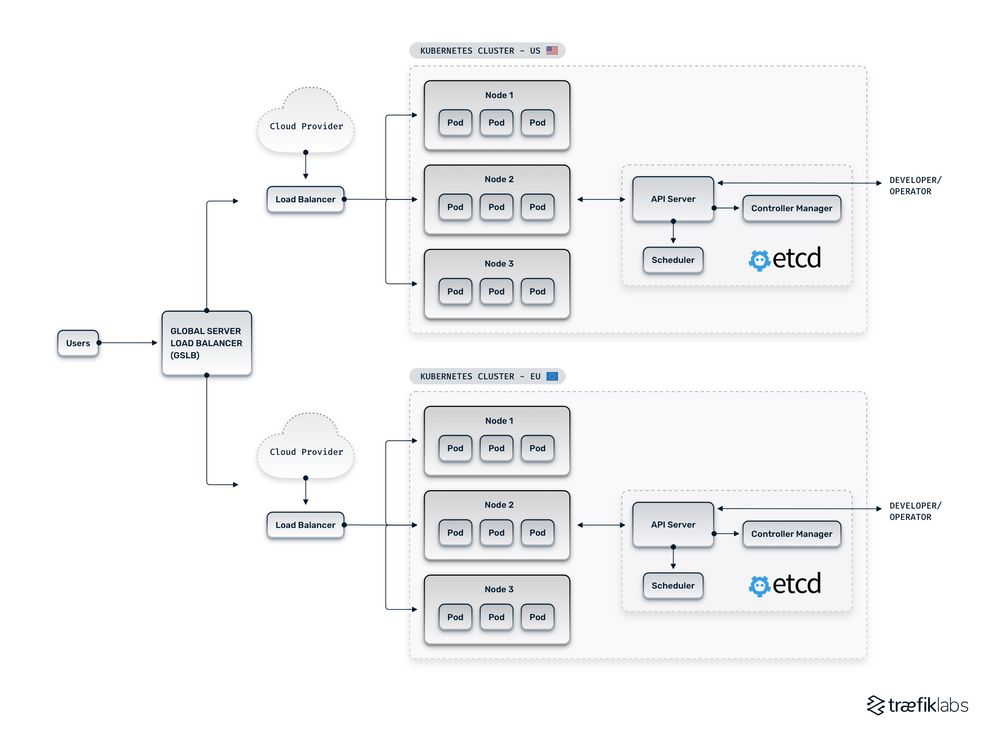
\includegraphics[width=1.0\textwidth]{figures/istio/multicluster.png}
          \caption{CSERE Multi-cluster architektúra bemutatása \cite{multicluster}.}
           \label{multi-cluster}
\end{figure}

A multi-cluster-es architektúra legegyszerűbb formájában nem tűnik olyan bonyolultnak és ijesztőnek.
A valóságban azonban többféleképpen lehet kialakítani egy multi-cluster-es Kubernetes-architektúrát.
Az architekturális választás a két fő architekturális megközelítésen alapul - szegmentáció vagy replikáció \cite{multicluster}.

\subsection{Több klaszteres architektúra tervek}
A szegmentációs megközelítéssel az alkalmazást független komponensekre tagolják, amelyeket általában Kubernetes-szolgáltatásokként ábrázolnak, és üzemeltetési követelményeknek megfelelően különböző Kubernetes-klaszterekhez rendelnek hozzá.
A replikációs megközelítéssel egy Kubernetes cluster pontos másolatai több adatközpontban, különböző helyszíneken vannak elhelyezve.
Ez redundanciát biztosít, így az alkalmazás elérhető marad abban az esetben is, ha az egyik cluster elérhetetlenné válik \cite{multicluster}.

\subsection{Kubernetes-központú vs. hálózat-központú konfiguráció}
A multi-cluster-es Kubernetes környezetek kezelésének két alapvető módszere van - Kubernetes-központú és a hálózat-központú.
Ha a Kubernetes-központú módszert használjuk a multi-cluster-es környezet kezelésére, akkor különböző alkalmazások futnak különböző Kubernetes cluster-eken, mégis mindegyiket egy központi helyről kezelik.

A hálózat-központú módszerrel az alkalmazás pontos másolatát több, különböző helyen lévő cluster-eken telepíti.
Bár ezek a cluster-ek különálló egységként viselkednek, az összes Kubernetes-cluster között egy hálózaton keresztül fenntartja a kommunikációt \cite{multicluster}.

\subsection{A több klaszteres architektúra előnyei}
Minden architektúra központi eleme az egyes cluster-ek függetlensége, és ebben rejlik a multi-cluster-es Kubernetes-architektúra nagy előnye.
A multi-cluster-es Kubernetes valós előnyeinek köre azonban ezen túlmutat \cite{multicluster}.

\subsubsection*{Rugalmasság}
A multi-cluster jelentős rugalmasságot és irányítást biztosít a tervezés és a konfiguráció megválasztása terén.
Például a Kubernetes különböző verzióit vagy disztribúcióit használhatja a különböző cluster-ekben, hogy megfeleljen az alkalmazások különböző részeire vonatkozó különleges igényeknek vagy követelményeknek.
A több multi-cluster-es architektúrával a Kubernetes különböző vagy újabb verzióit is tesztelheti elszigetelt cluster-ekben, mielőtt frissítené a produktív környezetét, így minimálisra csökkentheti a hibás változtatások és a leállások kockázatát \cite{multicluster}.

\subsubsection*{Elérhetőség, skálázhatóság és erőforrás-kihasználás}
A multi-cluster-es telepítések egyik legnagyobb előnye a Kubernetes teljesítményének javítása, különösen a rendelkezésre állás és a skálázhatóság tekintetében.
A multi-cluster-es architektúrával a munkaterheléseket a cluster-ek között mozgathatja.
Egy cluster-t használhat biztonsági mentésként, és a cluster-ek különböző adatközpontokban, helyszíneken és felhőkben is szétoszthatja.
Ezzel pedig minimálisra csökkentheti annak kockázatát, hogy egyetlen cluster meghibásodása miatt az egész környezete leálljon.
A cluster-ek különböző helyszíneken történő telepítésével csökkenti az alkalmazást tároló cluster és a végfelhasználó közötti fizikai távolságot, növelve ezzel a teljesítményt és minimalizálva a késleltetést.
A különböző cluster-ek között elosztott munkaterhelések nagyobb skálázhatóságot is eredményeznek.
A multi-cluster-es Kubernetes lehetővé teszi, hogy a különböző cluster-eket az adott terhelésüknek megfelelően fel- és lefelé skálázza - ez optimalizálja az erőforrás kihasználtságot az erőforrások különböző teljesítménykövetelményekhez való igazításával \cite{multicluster}.

\subsubsection*{Feladat izoláció}
Az elszigeteltség bizonyos szintje még egy cluster-es architektúrában is elérhető a névterek használatával.
Az egy cluster-es forgatókönyvben azonban a Kubernetes biztonsági rendszerének sajátosságai miatt a környezetek nem tökéletesen elszigeteltek egymástól.
A cluster-en belüli elszigetelés ezen módszerének használata esetén az azonos hardveren osztozó alkalmazások hatással lehetnek egymásra - ez a "zajos szomszéd" problémaként is ismert.
A munkafeladatok több Kubernetes cluste-en keresztüli futtatásával magas szintű elszigeteltséget eredményezhet.
Az esetleges cluster hibák vagy konfigurációs változások csak az adott cluster-t érintik.
A munkaterhelés-elszigetelés kulcsfontosságú a fejlesztőcsapatok számára, mivel segít nekik a problémák egyszerű elkülönítésében és diagnosztizálásában, az új funkciók és konfigurációk tesztelésében, az alkalmazások fejlesztésében és frissítésében, és mindezt úgy, hogy közben a produktív környezet biztonságos és elérhető marad \cite{multicluster}.

\subsubsection*{Biztonság és megfelelés}
A multi-cluster-es architektúra által biztosított magas szintű terheléselkülönítéssel minimálisra csökkentheti annak kockázatát, hogy az egymástól független alkalmazások nem kívánt módon lépjenek kölcsönhatásba egymással.
A szigorú elszigeteltség csökkenti annak kockázatát is, hogy az egyik cluster-ben felmerülő biztonsági probléma az egész környezetet befolyásolja.
Ez bizonyos mértékig egyetlen Kubernetes cluster-en belül is megvalósítható, például pod biztonsági házirendek használatával.
De semmi sem hasonlítható a multi-cluster-es Kubernetes által biztosított magas szintű teherelkülönítéshez.
A multi-cluster-es telepítések megkönnyítik a különböző országok eltérő szabályainak és irányelveinek való megfelelést is.
Erre remek példa az általános adatvédelmi rendelet (későbbiekben GDPR) az EU-ban.
A GDPR előírja, hogy a felhasználói adatok ne hagyják el az EU-t.
Ha világszerte vannak felhasználói és egyetlen cluster-ben futtatja az alkalmazást, akkor szinte lehetetlen lenne megfelelni ezeknek a követelményeknek.
A multi-cluster-es telepítésekkel egy cluster-t telepíthet az EU-ban, hogy megfeleljen ezeknek az igényeknek és a helyi előírásoknak, miközben máshol más cluster-eket futtathat \cite{multicluster}.

\subsection{A több klaszteres Kubernetes kihívásai}
Nagyon kevés jó dolog van az életben, amihez nem kell akadályokat leküzdeni, és a Kubernetes biztosan nem tartozik ezek közé.
A végtelen lehetőségek és a multi-cluster-es telepítésekkel járó fontos előnyök ellenére van néhány kihívás.
A Kubernetes nagyon összetett, a multi-cluster-es Kubernetes pedig még összetettebb. A hozzáadott komplexitás számos formában jelentkezhet \cite{multicluster}.

\subsubsection*{Konfiguráció}
Az architektúra kialakításától függően a környezet különböző cluster-i különböző konfigurációkat igényelnek az egyes cluster-ek sajátos igényeinek kielégítésére.
Ez aprólékos munka, és ezt nem lehet megkerülni. Ugyanennek a problémának egy másik szintje a tűzfal konfigurációja.
Az egy cluster-es architektúrában egyetlen API-kiszolgálót lehet elérni egy adott címen.

Multi-cluster-es telepítés esetén több API-kiszolgálót ér el de gondoskodnia kell arról, hogy a tűzfal lehetővé tegye a kapcsolódó cluster-ekben lévő API-kiszolgálók elérését.
Ennek enyhítésére automatizálási szkripteket használhat, amelyek sajnos szintén növelik a bonyolultsági szintet \cite{multicluster}.

\subsubsection*{Biztonság}
multi-cluster-es Kubernetesben a munkaterhelés elkülönítése segíti a jobb biztonsági helyzetet, de ennek eléréséhez figyelembe kell vennie az egyes cluster-ekre vonatkozó eltérő szabályokat és biztonsági tanúsítványokat.
Ahhoz, hogy megfeleljen a különböző helyi szabályozásoknak, ezeket a biztonsági tanúsítványokat különböző adatközpontokban és cluster-eken kell kezelnie \cite{multicluster}.

\subsubsection*{Telepítés}
Természetesen a multi-cluster-es Kubernetes architektúrában a telepítések egyre összetettebbé válnak.
Ez különösen igaz a GitOps megközelítés használata esetén. A GitOps-ban a forráskódkezelő szolgáltatása az összes telepítési tevékenység egyetlen forrása.
Ez azt jelenti, hogy a GitOps folyamatainak jól szervezettnek, biztonságosnak és intelligensnek kell lenniük.
A GitOps segíthet automatizálni a cluster-ek konfigurálását, képessé tesz a Kubernetes- cluster-ek életciklusának irányítására és a skálázott telepítésre \cite{multicluster}.

\subsubsection*{Költség}
Egy másik kihívás, amelyet a multi-cluster-es Kubernetes architektúra bevezetésekor figyelembe kell venni, a költségek potenciálisan jelentős növekedése.
A multi-cluster több node-ot jelent, ami viszont az erőforrás-felhasználás és végső soron a költségek növekedését eredményezi.
Egy másik fontos szempont, amit szem előtt kell tartani, a megnövekedett számú terheléselosztók, ingresszek, valamint naplózási és felügyeleti erőforrások szükségessége \cite{multicluster}.